\documentclass[10pt,twocolumn]{article}
% Main text. supplement.tex is a separate document with the same look; Folio
% builds both and shows the supplement after the paper. Each reads the
% other's labels: supplement labels are S-... here, main-text labels are M-...
% there. Export without the supplement turns every S-... reference into text.

\usepackage[margin=1.9cm,columnsep=0.6cm]{geometry}
\usepackage{lineno}               % add \linenumbers to the body for review copies
\usepackage{graphicx}
\usepackage{booktabs}
\usepackage{array}
\usepackage{longtable}
\usepackage{amsmath}
% Helvetica for all text with pdfLaTeX, its TeX Gyre Heros clone with XeLaTeX
% or LuaLaTeX; mathastext, loaded after it, sets math letters and digits in
% the same face, so inline math does not switch to a serif font.
\usepackage{iftex}
\ifPDFTeX
  \usepackage[T1]{fontenc}
  \usepackage{helvet}
  \usepackage{courier}
  % Unicode characters pdfLaTeX does not know; add more as sources need them.
  \DeclareUnicodeCharacter{2212}{\textminus}
  \DeclareUnicodeCharacter{2265}{\ensuremath{\geq}}
  \DeclareUnicodeCharacter{2264}{\ensuremath{\leq}}
  \DeclareUnicodeCharacter{2248}{\ensuremath{\approx}}
  \DeclareUnicodeCharacter{03B1}{\ensuremath{\alpha}}
  \DeclareUnicodeCharacter{2009}{\,}
\else
  \usepackage{fontspec}
  % By file name, so the fonts shipped with TeX Live are found on every system.
  \setsansfont{texgyreheros}[Extension=.otf, UprightFont=*-regular,
    BoldFont=*-bold, ItalicFont=*-italic, BoldItalicFont=*-bolditalic]
  \setmonofont{texgyrecursor}[Extension=.otf, UprightFont=*-regular,
    BoldFont=*-bold, ItalicFont=*-italic, BoldItalicFont=*-bolditalic]
\fi
\renewcommand{\familydefault}{\sfdefault}
\usepackage[italic]{mathastext}
\usepackage{rotating}
\usepackage{caption}

% xr-hyper before hyperref; cleveref after it.
\usepackage{xr-hyper}
\usepackage[hidelinks]{hyperref}
% Links stay clickable but uncoloured; URLs are set in Courier.
\renewcommand{\UrlFont}{\ttfamily}
\usepackage{cleveref}
\externaldocument[S-]{supplement}
\usepackage[super,sort&compress]{natbib}
\usepackage{authblk}
\usepackage{xcolor}
\usepackage{tikz}
\usetikzlibrary{positioning,calc,arrows.meta}
% Supplementary Notes: numbered, so they can be cited with \ref and \cref.
\newcounter{suppnote}
% Full, capitalised names (plain cleveref would print "fig." / "table").
% Supplementary items are cited as "Supplementary \cref{S-...}".
\crefname{figure}{Figure}{Figures}
\crefname{table}{Table}{Tables}
\crefname{suppnote}{Note}{Notes}
% Visible placeholder for information the authors still need to supply.
\newcommand{\tbd}[1]{\textcolor{red}{[#1]}}

\graphicspath{{figures/}}

% Two-column articles default to \flushbottom, which stretches the space
% between paragraphs and around headings to fill every column; let columns
% end naturally instead, and tighten heading spacing.
\raggedbottom
% Many journals (e.g. the Nature portfolio) do not number sections; remove
% this line for numbered ones.
\setcounter{secnumdepth}{0}
\usepackage{titlesec}
\titlespacing*{\section}{0pt}{2.2ex plus .5ex minus .2ex}{1.0ex plus .2ex}
\titlespacing*{\subsection}{0pt}{1.8ex plus .4ex minus .2ex}{0.8ex plus .2ex}
\titlespacing*{\paragraph}{0pt}{1.0ex plus .3ex minus .2ex}{0.8em}

% Let tall single-column figures share a column with text instead of being
% pushed onto their own float column.
\renewcommand{\topfraction}{0.9}
\renewcommand{\bottomfraction}{0.8}
\renewcommand{\textfraction}{0.07}
\renewcommand{\floatpagefraction}{0.8}
\renewcommand{\dbltopfraction}{0.9}
\renewcommand{\dblfloatpagefraction}{0.8}

\title{Title of the paper}
\author[1]{First Author}
\author[2,*]{Second Author}

\affil[1]{Department, Institution, Country}
\affil[2]{Department, Institution, Country}

\affil[*]{Corresponding author: \texttt{author@example.org}}

\begin{document}
\maketitle

\begin{abstract}
State the problem, what was done, the main results with their numbers, and
what they mean, in one paragraph. \tbd{Replace with the abstract.}
\end{abstract}

\section{Introduction}
Motivate the problem and what is missing in prior work~\cite{example2024article,example2023book}.
State the aim of the study in the last paragraph.

\section{Results}
% Figures are exported to figures/ as PDF (for example by an analysis
% script) and included by name; \graphicspath points there.
\begin{figure*}[htbp]
\centering
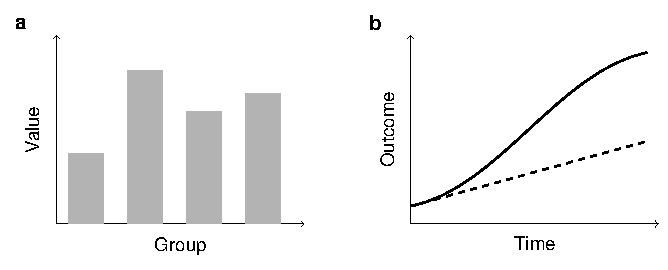
\includegraphics[width=0.7\textwidth]{example.pdf}
\caption{Study overview. \textbf{a}, What the first panel shows.
\textbf{b}, What the second panel shows.}
\label{fig:overview}
\end{figure*}

\paragraph{Main finding.} Describe the main result with its estimate and
interval (\cref{fig:overview}a, \cref{tab:results}). Details are in
Supplementary \cref{S-tab:supp-details} and Supplementary
\cref{S-fig:supp-flow}, and the additional analysis in Supplementary
\cref{S-note:supp-method}.

% Tables live in tables/, one file per table, so scripts can regenerate them.
\begin{table}[htbp]
\centering
\footnotesize
\caption{Main results. Estimates with 95\% confidence intervals (CI).
\textbf{Bold}: \textit{p}\textsubscript{adj}\,<\,0.05.}
\label{tab:results}
% Shrinks the table to the column width only when it is wider.
\resizebox{\ifdim\width>\columnwidth \columnwidth\else\width\fi}{!}{%
\begin{tabular}{lcc}
\toprule
\textbf{Method} & \textbf{Estimate (95\% CI)} & \textbf{Adjusted p} \\
\midrule
Proposed & \textbf{0.62 (0.60--0.63)} & <0.001 \\
Baseline & 0.33 (0.32--0.34) & -- \\
\bottomrule
\end{tabular}}
\end{table}


\paragraph{Secondary finding.} Describe it the same way (\cref{fig:overview}b).

\section{Discussion}
Summarize the findings, compare them with prior work~\cite{example2024article},
and state the limitations and implications.

\section{Methods}

\subsection{Data}
Describe the data sources and the reference standard.

\subsection{Statistical analysis}
Describe the models; the full specifications are in Supplementary
\cref{S-tab:supp-details}. For example, the estimate is
\begin{equation}
\hat{\theta} = \frac{1}{n}\sum_{i=1}^{n} x_i .
\label{eq:estimate}
\end{equation}

\section*{Data availability}
\tbd{Where and how the data can be accessed.}

\section*{Code availability}
\tbd{Repository URL, e.g.\ \url{https://example.org/code}.}

\section*{Acknowledgments}
\tbd{Funding and acknowledgments.}

\section*{Author contributions}
\tbd{Contributions of each author.}

\section*{Competing interests}
The authors declare no competing interests.


% naturemag gives numbered superscript citations; use unsrtnat or plainnat
% for author--year with natbib's other options.
\bibliographystyle{naturemag}
\bibliography{references}

\end{document}
